\chapter{OMMEB Alge Dump}

\section{Nivel 1}

\begin{problem}[OMMEB 2017]
    Los diez dígitos: 0, 1, 2, 3, 4, 5, 6, 7, 8, 9 se han 
    colocado cada uno dentro de un círculo de manera que las 
    dos sumas, de los seis números en cada hexágono, son iguales. 
    ¿Cuál es el valor de $b + c - a$?
\end{problem}

\begin{figure}[h]
    \centering
    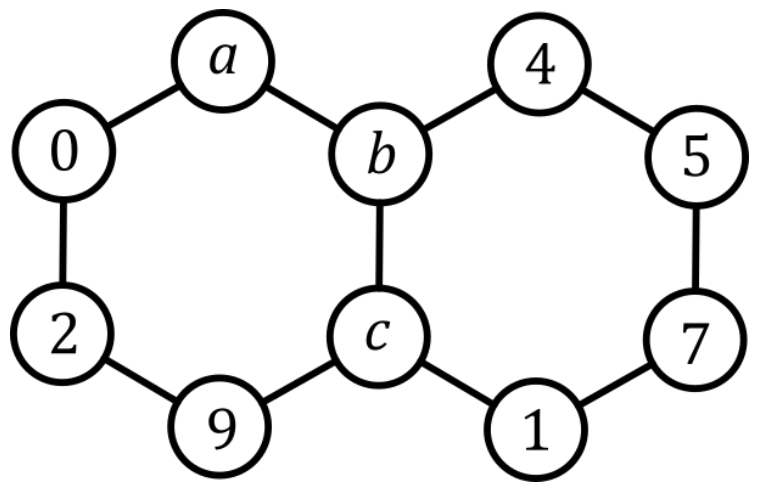
\includegraphics[height=3cm]{17OMMEBN1P1}
\end{figure}

\begin{problem}[OMMEB 2017]
    En la siguiente operación cada letra representa un dígito 
    entre 0 y 9. ¿Cuánto vale la suma $o+m+m+e+b$?
\end{problem}

\begin{center}
    \begin{tabular}{cccc}
        $o$ & $m$ & $m$ & $e$ \\
        + & $b$ & 3 & 1 \\
        \hline
        2 & 0 & 1 & 7 \\
    \end{tabular}
\end{center}

\begin{problem}[OMMEB 2017]
    Víctor y Vicky compraron un pastel y se lo comieron de la 
    siguiente manera: Una mañana Víctor se comió la mitad del 
    pastel, por la noche Vicky se comió la mitad del pastel que 
    quedaba. Este proceso siguió de lamisma manera durante 4 días, 
    comiendo cada uno la mitad del pastel que encontraban. 
    En la mañana del quinto día, Víctor se comió lo que quedaba 
    del pastel. ¿Qué proporción del pastel comió Víctor en los 5 
    días?
\end{problem}

\begin{problem}[OMMEB 2017]
    A Pedro y a María les dejaron de tarea recortar círculos de 
    cartón en fracciones. María recortó cada círculo en \(8\) 
    partes. Pedro las recortó en \(6\) partes. En total recortaron 
    \(30\) círculos y María terminó con el doble de piezas que 
    Pedro; ¿cuántos círculos recortó María?

\end{problem}

\section{Nivel 2}

\begin{problem}[OMMEB 2017]
    Los enteros positivos \(a, b, c, d, e\) cumplen con:
    \[
    a + \frac{1}{b + \frac{1}{c + \frac{1}{d + \frac{1}{e + 1}}}} = \frac{268}{187}.
    \]
    Encuentra el valor de \(a + b + c + d + e\).
\end{problem}

\begin{problem}[OMMEB 2017]
    Encuentra todos los enteros positivos \(x\), 
    que cumplan la ecuación 
    \[
    x^3 - 2017x - 360 = 0.
    \]
\end{problem}

\begin{problem}[OMMEB 2017]
    Al realizar la multiplicación \((x + 1)(x + 2)(x + 3) \cdots (x + 2017)\), 
    ¿cuál es el coeficiente de \(x^{2016}\)?
\end{problem}

\begin{problem}[OMMEB 2017]
    Los nadadores Omar, Mario, Miguel, Edgar y Beto van a 
    competir en una carrera libre en una alberca de cinco 
    carriles tal como sigue:
    \begin{enumerate}
        \ii Beto no nada al lado ni Mario ni Edgar.
        \ii Omar nada en un extremo.
        \ii Miguel nada entre dos personas ninguna siendo Mario.
        \ii Edgar no está en los carriles \(2,\), \(3,\) ni \(5.\)
    \end{enumerate}
    Indica en qué carril está cada uno.
\end{problem}

\begin{problem}[OMMEB 2017]
    Determina la cantidad máxima posible triángulos cuyos 
    vértices estén entre algunos puntos donde intersecan seis 
    rectas sin estar sobre ellas.
\end{problem}

\begin{problem}[OMMEB 2017]
    Coloca números entre uno hasta ocho dentro caras del 
    octaedro regular cumpliendo condición: si cada vértice 
    tiene producto total igual entre cuatro caras tocando dicho 
    vértice entonces suma pareja opuesta será igual entre sí.
\end{problem}

\begin{figure}[h]
    \centering
    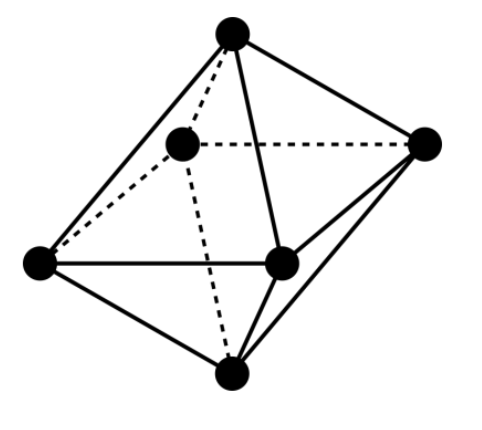
\includegraphics[height=3cm]{17OMMEBN2EP5.png}
\end{figure}

\begin{problem}[OMMEB 2017]
    Coloca números entre dos hasta ocho dentro círculos 
    cumpliendo condición si dos círculos están conectados no 
    pueden tener divisores comunes diferentes uno.
\end{problem}

\begin{figure}[h]
    \centering
    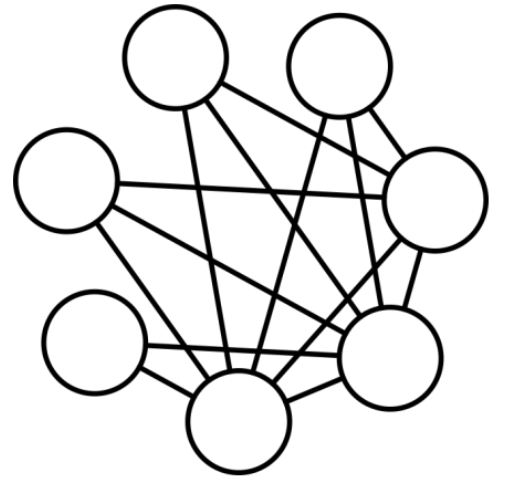
\includegraphics[height=3cm]{17OMMEBN3EP1.png}
\end{figure}

\section{Nivel 3}

\begin{problem}[OMMEB 2017]
    Por cada entero positivo n considera enteros positivos 
    $a$,$b$ tales: $ab=n$; donde no tienen divisores comunes 
    diferentes uno; además minimizando suma (si $n=ab=cd$ 
    entonces $a+b\le c+d$). Definimos $f(n)=\abs{s(a)-s(b)}$ 
    donde $s(j)$=suma dígitos $j$; calcular suma 
    \[f(1^2+1)+f(2^2+2)+...+f(2017^2+2017)\].
\end{problem}

\chapter{OMMEB Combi Dump}

\section{Nivel 1}

\begin{problem}[OMMEB 2017]
    Al imprimir un libro, el impresor no incluyó las hojas que 
    tienen páginas que terminan con la cifra \(8\). 
    Si el total de las cifras de las páginas que no se 
    incluyeron es \(230\); ¿cuál es el número máximo de páginas 
    que puede tener el libro original?
\end{problem}

\begin{problem}[OMMEB 2017]
    Se escriben en fila los números naturales a partir del 
    \(50\), excluyendo aquellos que tienen alguna cifra \(3\): 
    \(50515254555657585960616264 \ldots\). 
    ¿Qué cifra queda en el lugar \(2017\)?
\end{problem}

\section{Nivel 2}

\begin{problem}[OMMEB 2017]
    Un entero positivo se dice balanceado si todos sus dígitos 
    aparecen la misma cantidad de veces. Por ejemplo,
    \(1234, 101022\) y \(777\) son números balanceados. 
    Encuentra la cantidad de números balanceados menores a 
    \(10^4\).
\end{problem}

\section{Nivel 3}

\begin{problem}[OMMEB 2017]
    Sea P punto plano; dibujando n circunferencias radio uno tal P 
    sea común; encuentra máximo n sin tener centro alguna 
    circunferencia dentro/borde otra circunferencia.
\end{problem}

\chapter{OMMEB Geo Dump}

\section{Nivel 1}

\begin{problem}[OMMEB 2017]
    La siguiente figura está compuesta por el triángulo 
    equilátero \(ABH\); el rectángulo \(CDFG\) y el triángulo 
    isósceles \(DEF\); de manera que \(AB = DE\) y 
    \(CD = 2BC = 2GH\). Si el perímetro de \(DEF\) es \(8\) y 
    el perímetro de \(CDFG\) es \(10\), 
    ¿cuál es el perímetro de la figura?
\end{problem}

\begin{figure}[h]
    \centering
    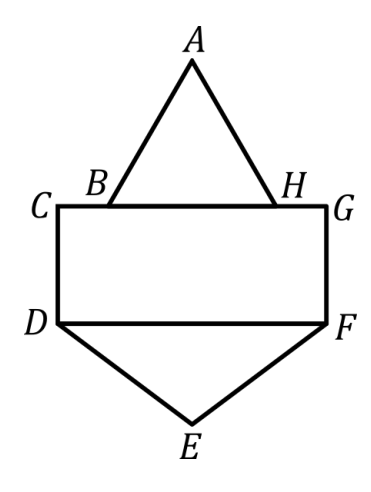
\includegraphics[height=4cm]{17OMMEBN1P5.png}
\end{figure}

\begin{problem}[OMMEB 2017]
    En la figura siguiente, la circunferencia mayor tiene radio 
    \(2\, cm\), ¿cuál es el área, en cm², de la región sombreada?
\end{problem}

\begin{figure}[h]
    \centering
    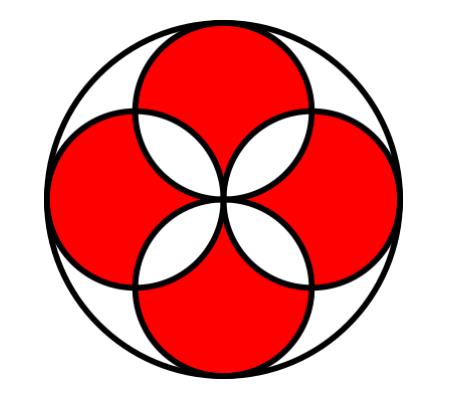
\includegraphics[height=3cm]{17OMMEBN1P10.png}
\end{figure}

\section{Nivel 2}

fumada y pitágoras (3-4-5)

\begin{sproblem}[OMMEB 2017]
    Las bases de un trapecio miden \(18\, cm\) y \(8\, cm\), y 
    los otros dos lados son \(8\, cm\) y \(6\, cm\). Encuentra 
    la longitud del segmento que une los puntos medios de las 
    bases.
\end{sproblem}

pitágoras y angle chasing

\begin{problem}[OMMEB 2017]
    Sea $ABCDEF$ un hexágono regular de lado \(2\, cm\). 
    Sea $P$ un punto dentro del hexágono tal que 
    $\angle APB$ = \(90^\circ\) y que $AP = PB$. 
    Encuentra el valor en $cm^2$ de $DP^2$.
\end{problem}

\begin{figure}[h]
    \centering
    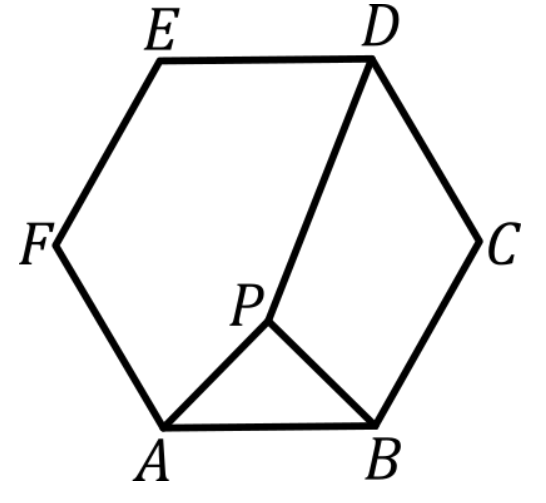
\includegraphics[height=3cm]{17OMMEBN1P15.png}
\end{figure}

semejanza y angle chasing

\begin{problem}[OMMEB 2017]
    En la siguiente figura, D es un punto sobre el arco AB, 
    los segmentos CA y CB son tangentes al arco en los puntos A 
    y B, respectivamente, y los puntos E, F y G son los pies de 
    las perpendiculares desde D a los lados AD, BC y CA, 
    respectivamente. Si DG = \(9\, cm\) y DF = \(4\, cm\), 
    calcula, en cm, la longitud DE.
\end{problem}

\begin{figure}[h]
    \centering
    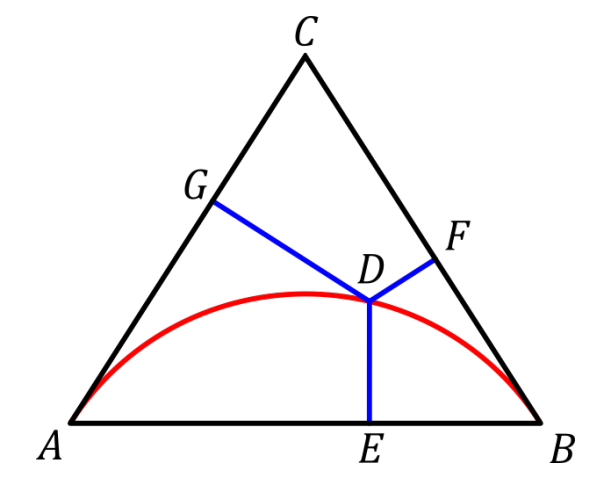
\includegraphics[height=3cm]{17OMMEBN2P10.png}
\end{figure}

razones, áreas y equiláteros

\begin{problem}[OMMEB 2017]
    Sean ABCD un cuadrado de lado \(\sqrt{2}\, cm\) y E, F 
    puntos tales que ACF y BDE son triángulos equiláteros.
    Encuentra la razón del área del cuadrilátero DCFE entre el 
    área del cuadrilátero ABFE.
\end{problem}

\begin{figure}[h]
    \centering
    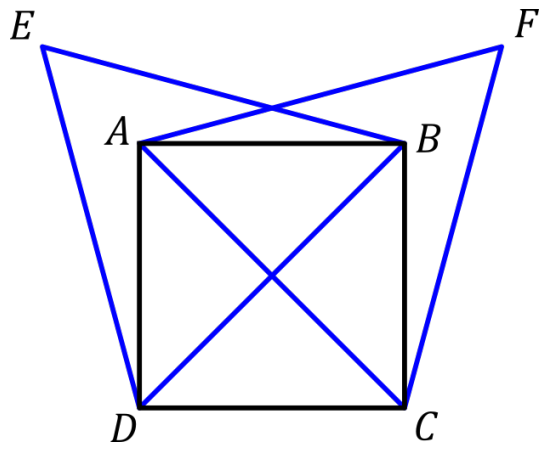
\includegraphics[height=3cm]{17OMMEBN2BP3.png}
\end{figure}

baricentro, fumada

\begin{problem}[OMMEB 2017]
    Las distancias desde los tres vértices A, B, C de un 
    triángulo ABC a una recta dada miden \(7\, cm\), \(9\, cm\) 
    y \(14\, cm\), respectivamente. Sean L y M los puntos medios 
    de BC y CA, respectivamente, y sea G el punto de 
    intersección de AL y BM. Calcula la distancia, en 
    centímetros, desde G a dicha recta.
\end{problem}

\begin{figure}[h]
    \centering
    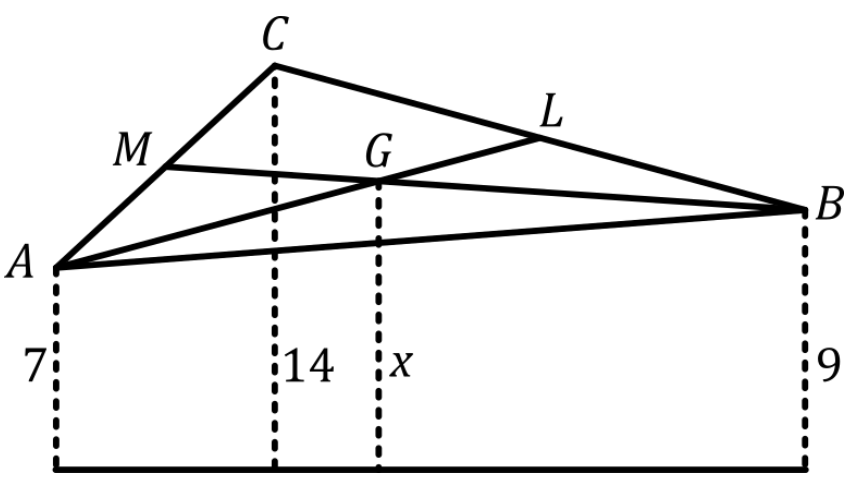
\includegraphics[height=3cm]{17OMMEBN3P2.png}
\end{figure}

áreas

\begin{problem}[OMMEB 2017]
    El diámetro FE mide \(4\,cm.\) Se divide en cuatro partes 
    iguales: FG = GH = HI = IE. Se trazan circunferencias con 
    diámetros FH , GI , HE . ¿Cuánto mide el área sombreada?
\end{problem}

\begin{figure}[h]
    \centering
    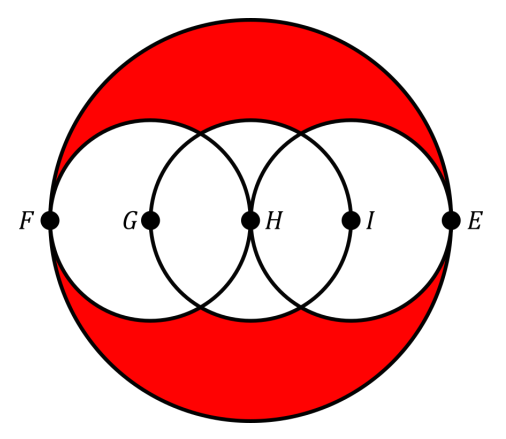
\includegraphics[height=3cm]{17OMMEBN1EP6.png}
\end{figure}

ángulos en circunferencia, congruencia SSA (por enseñar)

\begin{problem}[OMMEB 2017]
    Sea ABCD cuadrilátero circunscrito donde $AB>AD$; E punto 
    sobre lado $AB$ tal $BE=AD$; P punto sobre circunferencia 
    $C$ tal $AP=PE$ demuestra $\angle DCP=\angle PCB$
\end{problem}

\begin{figure}[h]
    \centering
    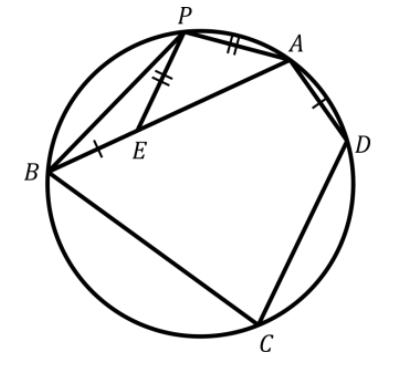
\includegraphics[height=3cm]{17OMMEBN2EP6.png}
\end{figure}

\section{Nivel 3}

triángulo especial 30-60-90, ángulos en circunferencia

\begin{problem}[OMMEB 2017]
    En el triángulo $ABC$, el segmento AB mide 1 cm, 
    $\angle BAC = 90^{\circ}$ y $\angle CBA = 60^{\circ}$. 
    Además $M$ y $N$ son los puntos medios de los arcos $AC$ y 
    $AB$ respectivamente en la semicircunferencia. Calcula, en 
    $cm^2$, el valor del área del triángulo $ANM$.
\end{problem}

\begin{figure}[h]
    \centering
    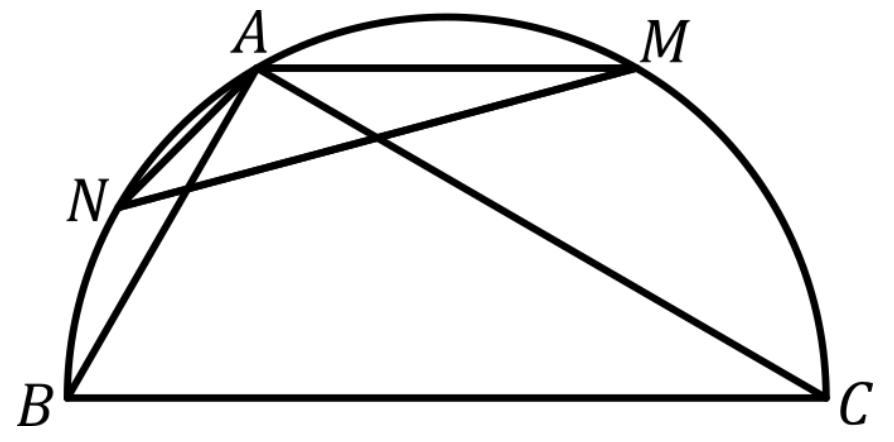
\includegraphics[height=3cm]{17OMMEBN3P12.png}
\end{figure}

intimida y ya

\begin{problem}[OMMEB 2017]
    Sean $A_1A_2A_3...A_{n-1}A_n$ y $A_1A_2B_3...B_nB_{n+1}$ 
    dos polígonos regulares con $n$ lados compartiendo lado 
    $A_1A_2$. Además $A_1A_2A_3...A_{n-1}A_n$ es interno a 
    $A_1A_2B_3...B_{n-1}B_nB_{n+1}$. Encuentra todos los valores 
    para $n>3$ tales que 
    \[
    \angle A_nB_{n+1}B_n= \frac{\angle A_1B_{n+1}B_n}{3}.
    \] 
\end{problem}

\chapter{OMMEB Nums Dump}

\section{Nivel 1}

\begin{problem}[OMMEB 2017]
    Si se lanzan \(3\) dados, calcula la probabilidad de que el 
    producto de los números que quedaron boca arriba tenga 
    exactamente dos divisores positivos.
\end{problem}

\begin{problem}[OMMEB 2017]
    Encuentra el máximo común divisor de \(111444444\) y 
    \(444111111\).
\end{problem}

\section{Nivel 2}

\begin{problem}[OMMEB 2017]
    El número \(10!\) tiene \(270\) divisores positivos. 
    ¿Cuál es la probabilidad de que al tomar uno de ellos al 
    azar, este divisor sea impar?
\end{problem}

\begin{problem}[OMMEB 2017]
    Encuentra la suma de todos los números positivos primos 
    relativos con \(100\) y que sean menores que \(100\).
\end{problem}

\begin{problem}[OMMEB 2017]
    Encuentre todos los números múltiplos por tres con cuatro 
    cifras sin usar las cifras dos o cuatro tales que al 
    dividirlos entre tres resulta otro número con las mismas 
    cifras originales pero ordenadas diferente.
\end{problem}

\begin{problem}[OMMEB 2017]
    El número donde vive Joaquín es el número \(932.\) Joaquín se 
    da cuenta que este número cumple las siguientes condiciones:
   \begin{enumerate}
    \item Todos sus dígitos son positivos.
    \item Aparecen en orden decreciente (\(9 > 3 > 2 >0.\))
    \item La suma entre su inversión (932+239=1171 ) resulta ser impar.
   \end{enumerate}
   ¿Cuáles números tienen estas propiedades?
\end{problem}

\section{Nivel 3}

\begin{problem}[OMMEB 2017]
    Encuentra todos los números de tres cifras que sean 
    cuadrados perfectos y tales que el número que se obtiene 
    al invertir el orden de sus cifras también sea un cuadrado 
    perfecto.
\end{problem}

\begin{problem}[OMMEB 2017]
    En un autobús van seis pasajeros, cada uno lleva un boleto 
    con número; los seis números son distintos. Además,
    los números de los boletos cumplen que ninguno es múltiplo 
    de cinco y para cada número hay exactamente otro, de los 
    cinco restantes, tal que ese par no tiene divisores positivos 
    en común, aparte del uno. ¿Cuál es el número más pequeño que 
    se puede obtener al multiplicar los números?
\end{problem}

\begin{problem}[OMMEB 2017]
    Los números enteros positivos a, b y c son distintos y 
    satisfacen:
    \[ 
    a|b + c + bc,
    b|c + a + ca,
    c|a + b + ab.
    \]
    Prueba que al menos uno de los números a, b o c no es primo.
\end{problem}

\begin{problem}[OMMEB 2017]
    El número natural M tiene exactamente seis divisores positivos 
    cuya suma es \(3500\). Encuentra todos los valores posibles para M.
\end{problem}

\begin{problem}[OMMEB 2017]
    Encuentra ternas enteras positivas (x,y,z ) cumpliendo 
    \[x^3+3x^2+z^2+2x+3y=2018\]
\end{problem}

\begin{problem}[OMMEB 2017]
    Por cada entero positivo n diferente cero termine escribe 
    dígitos inverso (ejemplo:2017*=7102); sea entero positivo menos 
    ocho dígitos tal a* diferente a; denotando D máximo común divisor 
    n/a* siendo mayor a 2017 dividiendo mínimo tres primos diferentes; 
    halla posible valor para a.  
\end{problem}

\begin{problem}[OMMEB 2017]
    Un entero positivo n bueno si exponente trece factorización 
    primos n! distinto cero divisible trece; encuentra enteros 
    positivos n buenos pero ninguno menor n-13 lo sea.
\end{problem}   
